% arara: latex: { interaction: nonstopmode, options: ['-halt-on-error'] }
% arara: dvisvgm: { options: ['--no-fonts', '--exact-bbox', '--zoom=-1'] }
\documentclass[tikz,border=8pt,11pt]{standalone}
\usepackage{amsmath}
\definecolor{circleblue}{HTML}{0072B2}
\definecolor{pointred}{HTML}{D55E00}
\definecolor{fixedpurple}{HTML}{8B4C9D}
\definecolor{ink}{HTML}{25313C}
\definecolor{muted}{HTML}{7C8792}
\tikzset{point label/.style={inner sep=4pt,text=ink}}

\begin{document}
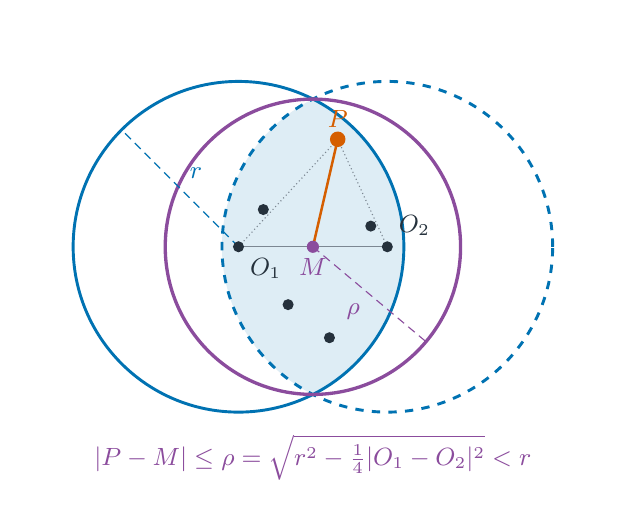
\begin{tikzpicture}[x=1.05cm,y=1.05cm,font=\small,text=ink]
  \fill[white] (-3.45,-3.1) rectangle (3.45,2.65);
  % The common lens is contained in the smaller disk centered at M.
  % r = 2, |O_1 O_2| = 1.8, so rho^2 = 4 - 0.9^2 = 3.19.
  \begin{scope}
    \clip (-0.9,0) circle[radius=2];
    \fill[circleblue!13] (0.9,0) circle[radius=2];
  \end{scope}
  \draw[circleblue,line width=1.05pt] (-0.9,0) circle[radius=2];
  \draw[circleblue,dashed,line width=1.05pt] (0.9,0) circle[radius=2];
  \draw[fixedpurple,line width=1.2pt] (0,0) circle[radius={sqrt(3.19)}];
  \draw[muted] (-0.9,0) -- (0.9,0);
  \draw[muted,densely dotted] (-0.9,0) -- (0.3,1.3) -- (0.9,0);
  \draw[pointred,line width=0.9pt] (0,0) -- (0.3,1.3);
  \draw[circleblue,densely dashed] (-0.9,0) -- (-2.3142,1.4142)
    node[midway,above right] {$r$};
  \draw[fixedpurple,densely dashed] (0,0) -- (1.3692,-1.1489)
    node[midway,below left] {$\rho$};
  \foreach \px/\py in {-0.3/-0.7,0.2/-1.1,-0.6/0.45,0.7/0.25}{
    \fill[ink] (\px,\py) circle[radius=2pt];
  }
  \fill[pointred] (0.3,1.3) circle[radius=2.8pt]
    node[point label,above,text=pointred] {$P$};
  \fill[ink] (-0.9,0) circle[radius=2pt]
    node[point label,below right] {$O_1$};
  \fill[ink] (0.9,0) circle[radius=2pt]
    node[point label,above right] {$O_2$};
  \fill[fixedpurple] (0,0) circle[radius=2.2pt]
    node[point label,below,text=fixedpurple] {$M$};
  \node[text=fixedpurple] at (0,-2.55)
    {$|P-M|\le\rho=\sqrt{r^2-\tfrac14|O_1-O_2|^2}<r$};
\end{tikzpicture}
\end{document}
